\documentclass[UTF8]{article}
\usepackage{ctex}[14pt,a4paper]
\usepackage{graphicx}
\usepackage[left=4.2cm,right=4.2cm,top=3.5cm,bottom=3.5cm]{geometry}
\usepackage{epstopdf}
\usepackage{float}
\usepackage{threeparttable}
\usepackage{subfig}
\usepackage{amsmath}
\usepackage{cases}
\usepackage{url}
\newcommand{\upcite}[1]{\textsuperscript{\textsuperscript{\cite{#1}}}}
\title{题目}
\date{}
\begin{document}

\section*{摘\quad 要}
\begin{flushleft}
这是一个信息大爆炸的时代,数字,文字,视频和音频都是信息。如何大量的数据中挖掘出我们感兴趣的具有指导意义的信息是至关重要的。构建了基于用户评论的评分模型。

为了了解消费者喜好与基本信息,我们利用Python里的自然语言处理库-TextBlob对产品评论的内容进行了词频统计和情感分析。我们发现评论数量呈指数增加,越来越多的消费者选择网上购物,其中美妆与婴儿用品更受消费者欢迎。Specific quality descriptors of text-based reviews such as ‘love’, ‘disappointed’, and others, strongly associated with rating levels.

为了了解产品声誉和预测产品是否推广成功,通过基于用户评论的评分模型,我们定义了产品声誉得分和产品未来发展得分。为了了解产品评价内容是否具有马太效应,我们用时间序列中的移动平均法算法对每个商品评价数量评论数的产品进行相关系分析,发现后面评论者的评论与前面评论者的评论具有相关性。

最后,我们进行敏感性分析并扩展模型。

		
		
\textbf{关键词:} {}
\newpage
\end{flushleft}





\section{问题重述}
\subsection{问题背景}
随着电子商务的发展,以及物流服务水平的提高,越来越多的人选择了网上
购物这种快捷方便的购物方式。伴随着着大数据的发展和数据的海量增加,数据在商业决策与公司发展中扮演者重要角色。顾客可以从他人的评价中获得信息从而决定是否购买;企业可以从大数据中发掘信息从而更好服务顾客,增加效益,提升行业竞争力。
\subsection{提出的问题}
为了使阳光公司的三个在线销售产品取得成功,首先我们要在已给定的唯一可使用数据中通过评论与评级识别相关的关键模式、关系、度量和参数。然后我们的两大目标是:1.明确销售策略;2.发现潜在的影响销售额的有助于提升产品满意度的重要特质。最后还应当充分考虑下来一系列要求;
\begin{itemize}
	\item 建立数据度量机制:一旦吹风机,微波炉,婴儿奶嘴在线销售后,该公司就能根据市场反应(评级,评论)来发现产品的顾客喜爱度,销售情况,值得提升的方面。
	\item 把时间因素考虑进去,建立基于时间的模型,能够讨论以后各商品的发展趋势,市场竞争力,以及市场声誉。
	\item 综合文本和评级的度量,预测产品是否会成功赢得市场喜爱。
	\item 考虑是否特定的某一个星级会引起更多其他人的相似评论。
	\item 一些特殊的词语是否与评级有强相关关系。
\end{itemize}

\subsection{问题分析}
首先我们要通过Python的自然语言处理库对评论进行情感分析,词频提取。然后建立模型对文本和数据进行感兴趣问题的数据挖掘,其中包括产品声誉,关键词,评论有效性,产品特质。最后给阳光公司一些在线销售策略。

\section{问题假设}
\begin{itemize}
	\item 假设用户购买商品就会发表一次评论,即可认为销量等价于评论的数量
	\item 假设Sunshine公司所给的产品数据集符合线上市场规律,即数据集所处的时间段中未发生异常状况,如自然灾害导致的产品销量上升或下降现象
	\item 假设认为数据集中用户在下订单和收到货物的时间间隔较小,即后不久就做了评论。
	\item 把订单中评级和评论内容有显著差异的订单看作正常订单
\end{itemize}

\section*{符号说明}
\begin{table}[H]
\centering

\begin{tabular}{lll}
	\hline
	符号\quad\quad\quad\quad\quad\quad\quad\quad\quad &意义  \\
	\hline 
	$ \mathbf{k}  $   &  评论得分
	\\
	$ \mathbf{s}  $   & 星级
	\\
	$ \mathbf{P}  $   & 极性分数,确定评论者对该产品是正面还是负面
	\\
	$ \mathbf{S}  $   & 主观性得分
	\\
	$  \mathbf{\beta_i} $   & 有用票比例
	\\
	$\mathbf{r}   $   & 评论的重要度
	\\
	$ (\boldsymbol{f1},\boldsymbol{f2},\boldsymbol{f3})  $   & 评论的有效分数,产品得分,消费者真实评价分数
	\\
	$  \mathbf{p} $   &每个评论者对该产品的声誉贡献分数
	\\
	$ \psi_j $   &  产品j未来发展得分
	\\
	$  \rho $   & Person相关系数
	\\	
	\hline
\end{tabular}
\end{table}

\section{模型1:单词频率算法}
\subsection{TF-IDF算法的简介与前期准备}

我们要确定每条评论的属性信息,就必须要先提取出该评论句中的有效信息,
再根据所提取出来的词语来对其进行判断。TF-IDF算法是一种统计算法,它能够统计某一个单词在某一篇文章中的出现次数,进而求得该单词出现的频率。我们用单词出现频率来刻画该单词在文章中的重要性。

在进行单词频率统计之前,我们还必须认识计算机是怎样将文章中的单词进行提取的。我们知道提取单词是一件非常繁琐的事,在此过程中我们要考虑到多种情况:
\begin{itemize}
	\item 一些简单词如$'a','an','is','the'\cdots$大量存在,又毫无分析意义,所以在进行自然语言处理时,不考虑这类单词,即停用词不考虑。
	\item 如$'like'$,$'Like'$,$likes$首字母大小写不同,单词时态不同的,本来应该看作一个单词,但在本文中把他们看作不同的词来进行分析。
	\item 用空格和标点符号对句子进行分割提取单词时,一些缩写词如$we'll$ ,$we're$,$pinkish-blue$本来是很难分割的,但在NKTL库能够对他们进行准确的分割。
\end{itemize}
Python有许多非常强大的自然语言工具包,能够用看起来简单但非常复杂的操作为我们节省大量的时间。在本文中我们选用NLTK来对文本数据继续单词频数与频率统计。在停用词的处理上,我们下载了一个停用词数据集\url{https://blog.csdn.net/shijiebei2009/article/details/39696523/},其中包括891个单词。在处理文本数据时候,我们在已分割的单词中删除了$891*2+1$种单词,这考虑到了停用词单词首字母大写和不明原因的空格符情况。

在单词频率算法中,我们之所以用NLTK库实现TF-IDF算法是因为NLTK库处理文本内容时可以对多个文本内容进入组合计算,而不是只能对单个文本进行计算。

\subsection{TF is Term Frequency}
TF 表示关键字在文本中出现的频率。为了防止它偏向较长的文本,这个数字通常会被归一化。值得一提的是在后文中出于其他考虑,我们也用到了单词频数。公式如下:
\begin{equation}
t f_{i j}=\frac{n_{i, j}}{\sum_{k}^t n_{k, j}}
\end{equation}
where:

$n_{i,j}$表示第i个词在文件$d_j$中出现的次数;

t表示文件$d_j$中所有词条的数目

分母则是文件$d_j$中所有词条的数目出现次数总和。

\subsection{ IDF is Inverse Document Frequency}
 TF-IDF的主要思想是:如果某个单词在一篇文章中出现的频率高,并且在其他文章中很少出现,则认为此词具有很好的类别区分能力,适合用来分类。如果包含词条t的文档越少, IDF越大,则说明词条具有很好的类别区分能力\upcite{Baenagarc2012TF}。这也符合我们想要对评价内容进行定性分析的目标。公式如下:
 \begin{equation}
 i d f_{i}=\log \frac{|D|}{\left|\left\{j: t_{i} \in d_{j}+1\right\}\right|}
 \end{equation}
 where:
 
 |D|表示所研究文本的个数;
 
 $j: t_{i} \in d_{j}$表示包含词条ti的文件数目。在此加1是为了避免分母为0的情况。
 
\subsection{Tf-idf is actually: TF * IDF}
某一特定文件内的高词语频率,以及该词语在整个文件集合中的低文件频率,可以产生出高权重的TF-IDF。因此,TF-IDF倾向于过滤掉常见的词语,保留重要的词语。公式为:
\begin{equation}
TF-I D F=T F * I D F
\end{equation}

\subsection{how to track sales situation form this modle}
通过对高频次出现次数和评论的了解,我们可以了解到消费者真正关心产品特质,还可以分析得到消费者关于产品和销售服务不满意的地方。阳光公司可以对这些地方进行改进与加强。

\section{模型2:基于用户评论的评价性模型}
\subsection{评论的定性分析}
现在的网络购物者们对商品好坏的定义各有千秋,但除非购物者对一件商品特别不满意,大多数时候都会给其好评,因为网络商品提供者没有门面费用等开销,导致网上的商品十分便宜,而人们对于一件便宜买到的商品往往会比较“口下留情”,这便使得后面想买该商品的用户看到的经常是“还好,还行,挺好的”之类的评论\upcite{zz}。评论的内容才是真正决定购买者真实想法的数据,我们需要从文本数据中挖掘出该产品真实的得分。

\begin{figure}[H]
	\centering
	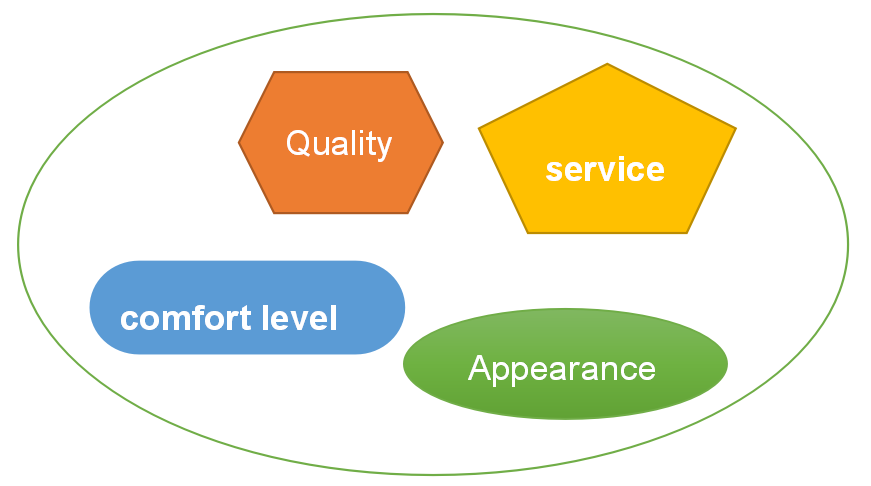
\includegraphics[width=6cm]{./figures/m1p.png}
	\caption{The main content of the product review} \label{m1p}
\end{figure}

图\ref{m1p}中可以知道,评论的主要内容包括四个方面:质量,服务,舒适度,外观。大量的评论还包括使用商品后的主观感受。所以要对商品进行情感分析。

TextBlob站在NLTK和pattern的巨大肩膀上,并且两者都很好地配合使用,并且可用于深入研究普通自然语言处理(NLP)任务,例如词性标记,名词短语提取,情感分析等\upcite{Martinc2015Efficient}。情感和主观性分类:这是学术界研究最多的领域。它将情感分析视为文本分类问题。已被广泛研究的两个子主题是:(1)将有观点的文件分类为表达正面或负面的意见,(2)将句子或句子的从句归类为主观或客观的,以及主观的句子或从句将其归类为表达正面,负面或中立的观点。情感分析旨在在经过评论的文本中找到作者的总体情感。例如,给定产品评论,它确定评论者对该产品的情感是正面还是负面。在本文中我们用到了情感分析得到了两个值:polarity,subjectivity。polarity表示极性分数在[-1.0,1.0]范围内浮动。主观性得分是在[0.0,1.0]范围内的浮动,其中0.0是非常客观的,而1.0是非常主观的。

本文将所有评论统一划分为5类进行分析:

1.  好评(纯好评,无任何说商品不好的言语);

2.  好评(整体好评,夹带一些不满);

3.  中评(较为客观的评价,观点居中);

4.  差评(因为某些意外或者服务态度,如快递原因);

5.  差评(因商品本身,如质量原因)。

按polarity对评论内容进行定性分析,得到评论得分:
\begin{equation}\label{m1gs1}
k_i=\left\{\begin{array}{lll}
1 & \text { bed review } & \text {if -1 $\leq$ polarity < 0 }\\
2 & \text { medium review } & \text {if polarity = 0 }\\
3 & \text { good review } & \text {if 0 < polarity $\leq$ 0 }
\end{array}\right.
\end{equation}
\begin{figure}[!htbp]
	\centering
	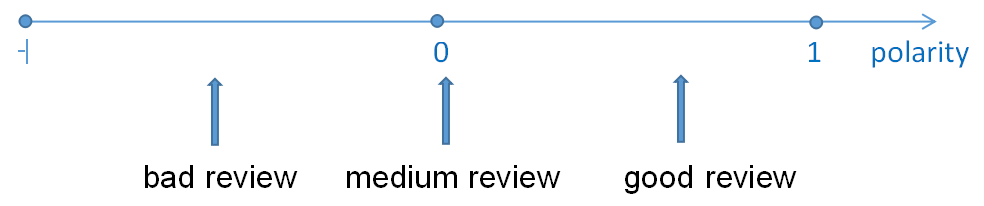
\includegraphics[width=8cm]{./figures/m11p.png}
	\caption{Attribute analysis of comment content} \label{m11p}
\end{figure}

$k_i$为评论得分,这是根据消费者的评价得到的。polarity表示极性分数在[-1.0,1.0]范围内浮动。polarity越接近于1表名消费者对产品的评价越好,polarity越接近于-1表名消费者对产品的评价越差。0代表消费者对产品的评论即不是消极评论,也不是积极评论,即为中评,评分为2 。

\subsection{评论的重要度}
评论的重要度体现在四个方面:

\begin{itemize}
	\item 有用票数占总票数的比例越大,则信息量更大。重要度加1;
	\item 如果该顾客的评级较高,是”绿标“的话,则影响力更大,重要度加2;
	\item 如果该顾客的评论越客观,即subjectivity越小,则评论越重要,重要度加1;
	\item 如果该顾客确实购买了产品,则评论可信度较高,重要度加1.
\end{itemize}

根据以上描述,得到评论的重要度:
\begin{equation}
r_{i}=\frac{\sum_{1}^{4}r_{ij}}{\mathbf{max} r_i}
\end{equation}

\begin{equation}
\beta_i=\left\{\begin{array}{ll}
\frac{helpful\quad votes}{total\quad votes} & \text { if total votes $\neq$ 0 } \\
0 & \text { else } 
\end{array}\right.
\end{equation}
其中:
$\beta_i$是有用票比例;

$
r_{i1}=\left\{\begin{array}{ll}
2 & \text { if $\beta_i$ > 50\% } \\
1 & \text { if $\beta_i \leq $50\% } \\
0 & \text { $\beta_i$ = 0 } 
\end{array}\right.
$
表示有用票的重要度属性;


$
r_{i2}=\left\{\begin{array}{ll}
2 & \text { if vine = Y } \\
0 & \text { else } 
\end{array}\right.
$
表示评论人的重要性属性;

$
r_{i3}=\left\{\begin{array}{ll}
1 & \text { if $S_i$ <0.5  } \\
0 & \text { else } 
\end{array}\right.
$
表示评论的客观程度属性;

$
r_{i4}=\left\{\begin{array}{ll}
1 & \text { if verified purchase = Y } \\
0 & \text { else } 
\end{array}\right.
$
表示评论者是否购买属性。

\subsection{不同信息的输出模型}
\begin{equation}\label{q1}
f(\boldsymbol{k},\boldsymbol{r},\boldsymbol{s})=(\frac{1}{3}\boldsymbol{k}^T\cdot \boldsymbol{r},\eta \boldsymbol{s} + 5(1-\eta)\boldsymbol{r},\phi\boldsymbol{s} + \frac{5}{3}(1-\phi)\boldsymbol{k})=(\boldsymbol{f1},\boldsymbol{f2},\boldsymbol{f3})
\end{equation}\label{zy1}
where:

$f1_i$表示评论的有效分数,范围在$[0,1]$之间.这即考虑到对文本进行情感分析所得评论得分,又考虑到评论的重要性。评论的有效得分是能够筛选出重要的评论,是给阳光公司提供客户意见时的重要依据。

$f2_i$表示产品得分,范围在$[0,5]$之间。能够综合反应产品的价值,质量。这对评价产品是否会成功或失败至关重要。因为有时候星级与评论是矛盾的,这是我们采用加权法来对两者进行协调。我们知道评论是手动输入的不可能违背消费者原本评价,而星级是鼠标点上去的,所以很可能会出错。出现星级为1或2,但评论则是好的这种情况。

为什么我们对星级与评论相矛盾的数据没有进行删除呢?

因为通过赛题给出数据,我们们发现2008年以前的数据都非常少。如果将原本少的数据再减少,这不利于数据分析。

$f3_i$表示消费者真实评价分数,范围在$[0,5]$之间。这能够反应消费者对购买产品的真实感受。

$\phi$表示星级占消费者真实评价分数的权重,$1-\phi$表示评论得分占消费者真实评价分数的权重。在消费者真实评价分数中,我们将星级与评价分数视为同等重要,所以$\phi=0.5$。

$\phi$表示星级占产品得分的权重,$1-\phi$表示评论得分占产品得分的权重。在产品得分中,评价有效得分看作比星级更重要的因素,所以$\eta=0.3$.

\subsection{how to track sales situation form this modle}
一旦三种产品在在线市场上销售后,阳光公司可以根据这三个数据来度量和跟踪产品的销售情况。阳光公司可以通过产品得分来了解商品质量等实质因素在消费者心中的优劣,也可以根据消费者真实评价分数确定该产品在消费者心目中的真实感受。

\section{问题结果与建议}
\subsection{inform online sales strategy}
首先我们对已知的原始数据做一些基本分析,了解在线销售的基本情况。提出了一系列阳光公司可能感兴趣的问题?

1.美国网购是不是越来越普遍?

2.在线销售是否会取代传统的市场销售?

3.在线销售和传统销售相比谁的用户体验更好?

4.什么产品适合在线销售?

5.消费者更关心产品的哪些方面?

\begin{figure}[h]
	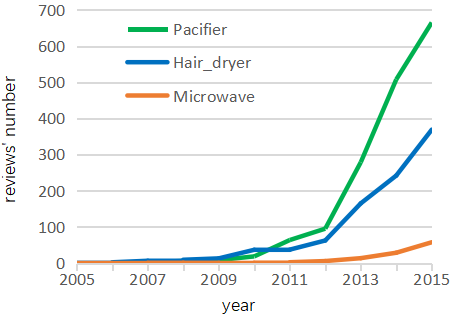
\includegraphics[width=7cm]{./figures/q1p1.png}
	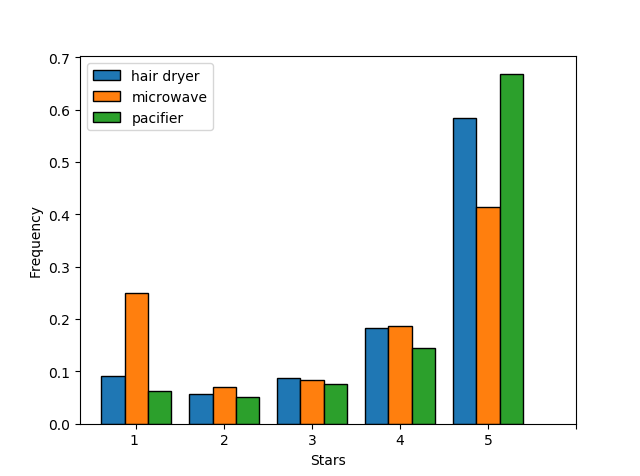
\includegraphics[width=7cm]{./figures/z1.png}
	\caption{左图:三种产品每一年的月平均评论个数;右图:三类产品所有数据星级频率} \label{z1_q1p1}
\end{figure}

我们知道评论个数与网上购物人数是成正比的,所以可将右图看作为网上购买人数与时间的关系。通过左图我们可以发现,在2008年以前选择在网上购物的人非常少,在2008年后网购变得越来越流行了。分析其中原因,2008年美国发生次贷危机,引发全球金融危机,导致很多银行倒闭,中小型企业受到冲击也倒闭,为了寻求生存,许多小型企业纷纷转战线上销售,因为众所周知线上销售成本小,不用租金,顾销售人员。

我们发现在2008年以后,网上购物人数呈指数增长,这表明网上购物越来越受顾客欢迎。我们有理由相信在线销售会打败传统的市场销售,网上购物会成为新时代人们购物的新习惯。在此强烈建议阳光公司开展网上销售业务。

安抚奶嘴属于婴儿用品类,电吹风属于美妆类,微波炉属于大型家电类。在左图中我们发现相比于电吹风与安抚奶嘴,微波炉评论数量非常少,即网上购买微波炉的人数较少。结合右图可以发现微波炉的一星是非常多大,这说明消费者不同喜欢在网上购买大型家电。综上所述,美妆和婴儿用品更适合网上销售。

右图是三类产品网上评论星级分布图,安抚奶嘴与吹风机五星出现的频率超过50\%,说明大多数人对这类产品的网上购物用户体验很好。大家都能买到即便宜又好用的东西,能满足自己的需求。

通过Python的NLTK用TF-IDF算法对评论内容进行词频统计,并通过wordcloud绘制如下的词云图。

\begin{figure}[H]
	\centering
	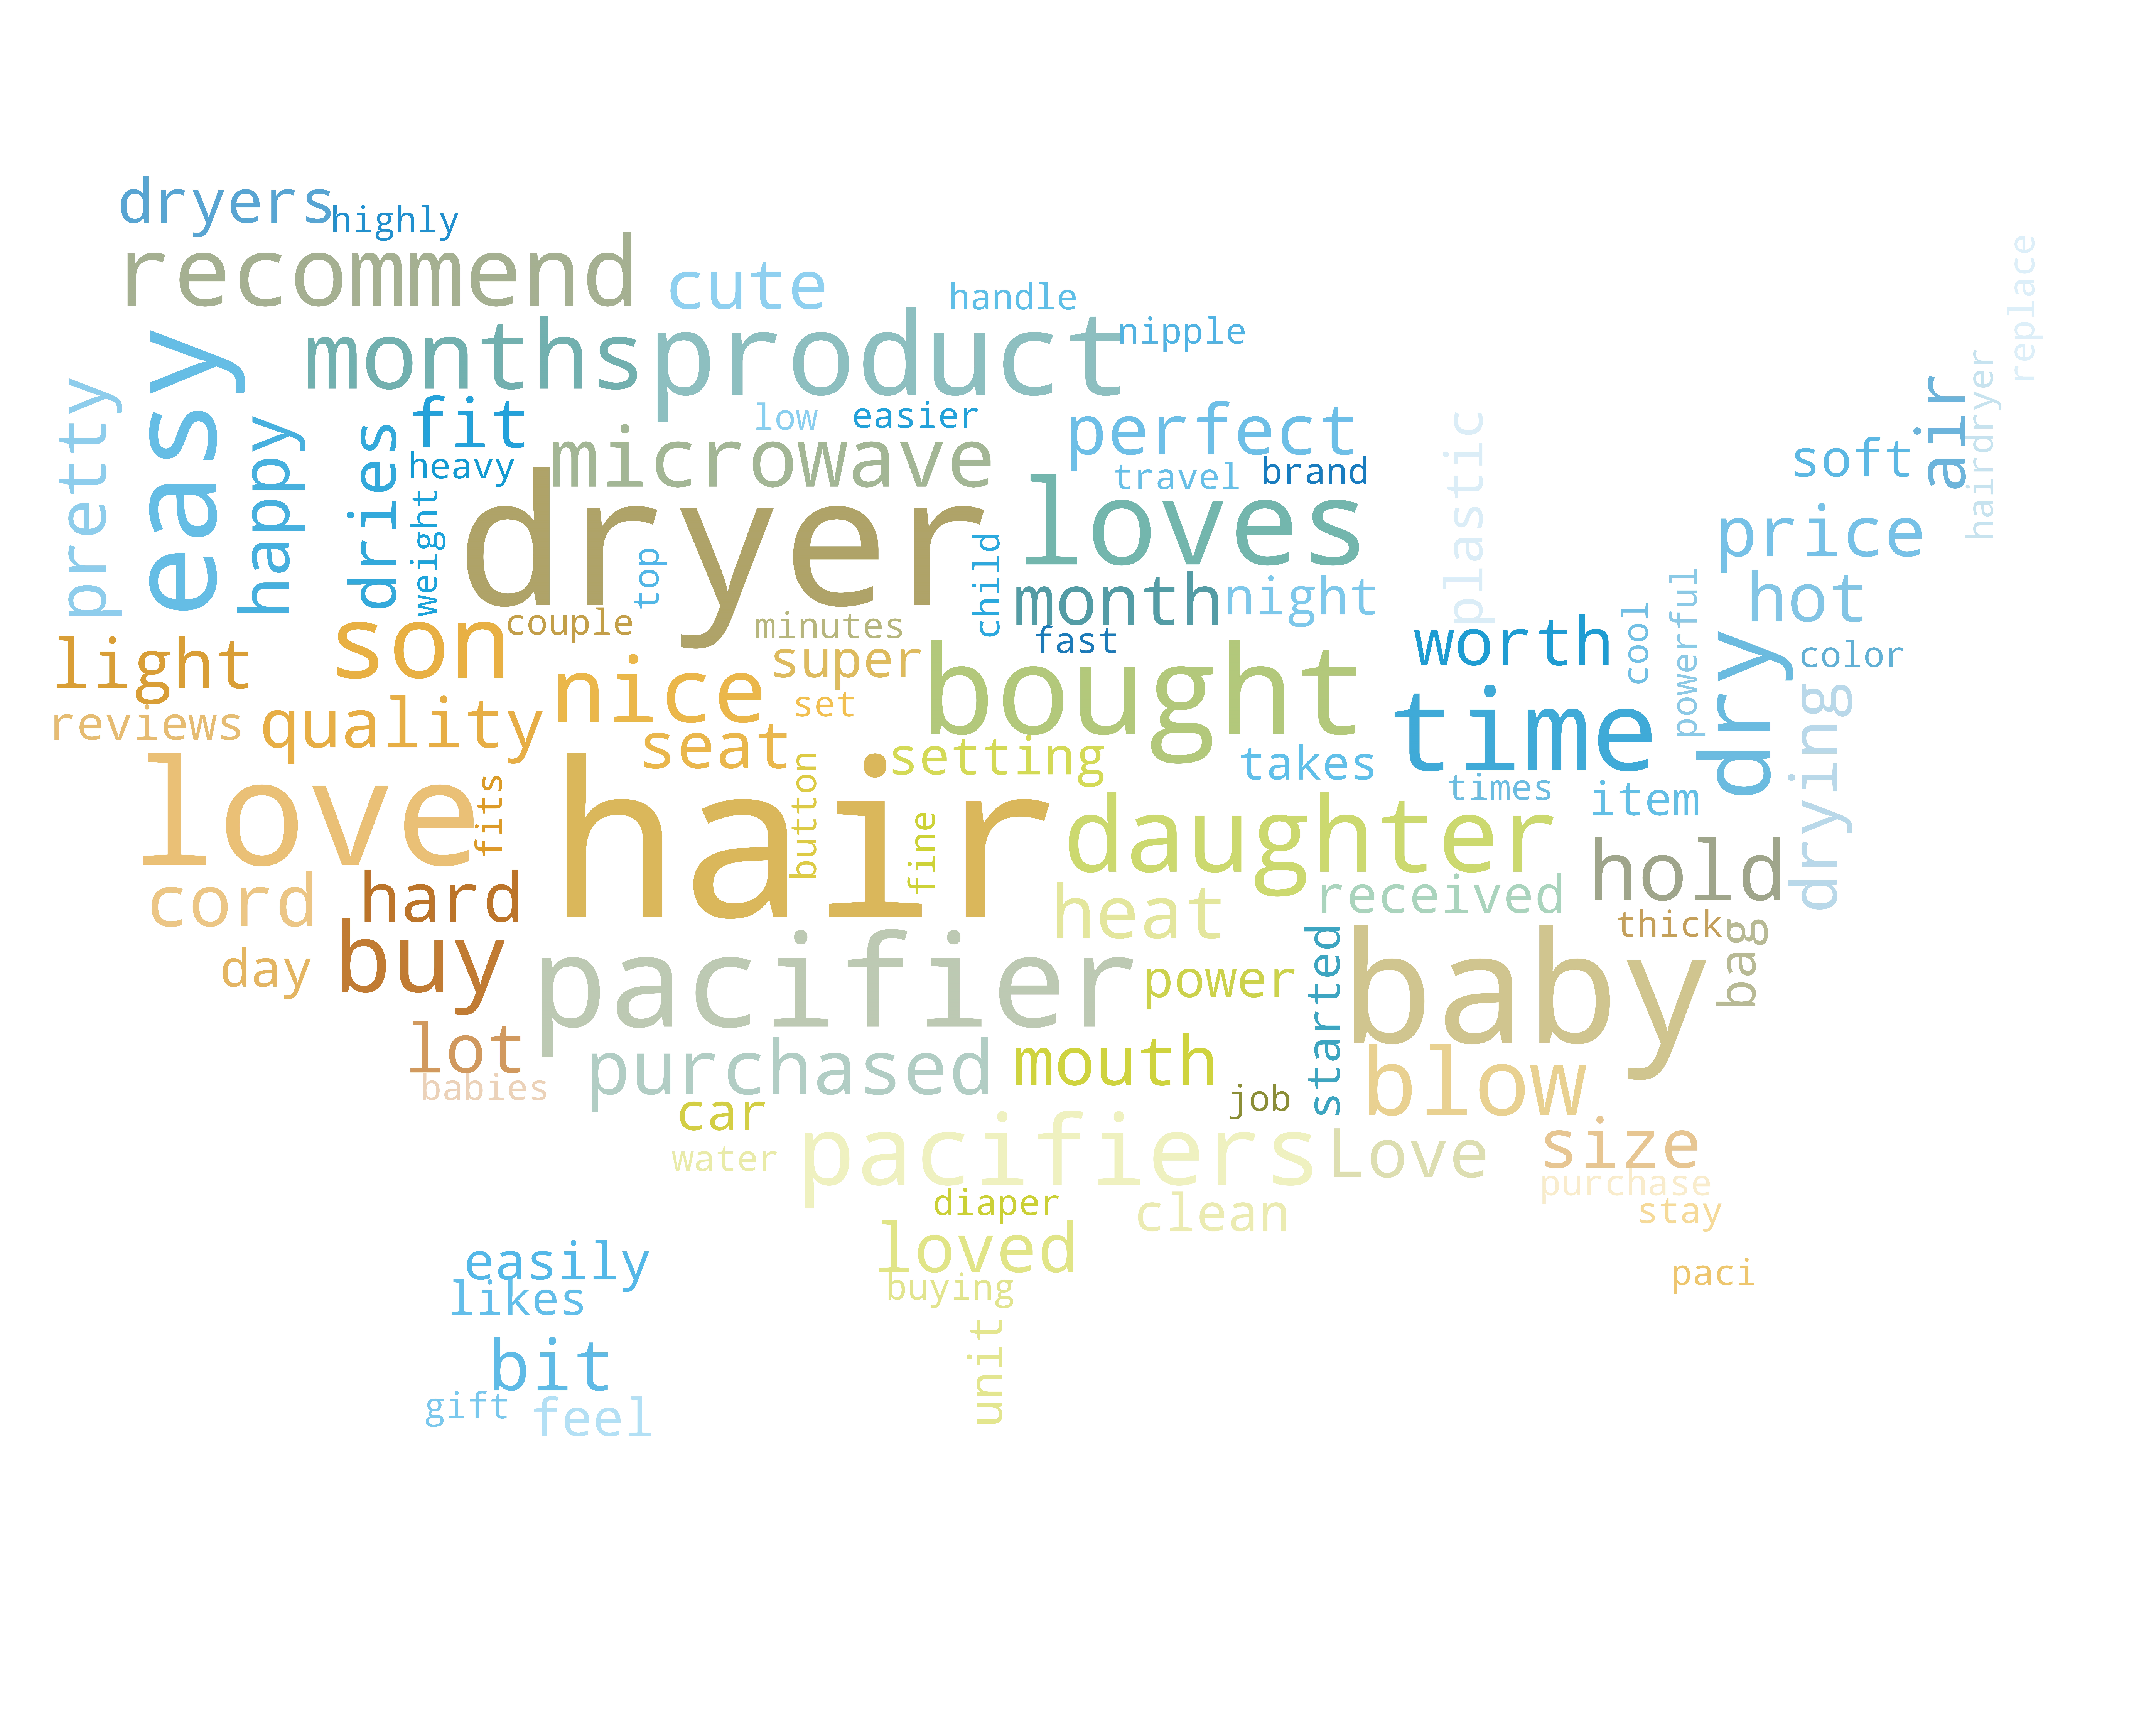
\includegraphics[width=8cm]{./figures/wc.png}
	\caption{三个数据集所有评论的词云图} \label{wordCloud}
\end{figure}
从图\ref{wordCloud}可知:消费者最关心产品的质量与价格,所有在在线市场上推出产品时,即要保证产品质量好,又要相当于同一类型产品而言价格"优美"。



\subsection{potentially important design features}
在对消费者评论的研究中,我们通过单词频率算法得到每类产品各星级对应的高频词汇。发现质量,服务与价格是最受消费者关心的。现在我们想了解具体产品潜在的重要设计功能,以增强产品的满意度。受篇幅限制,下面我们只给出婴儿奶嘴单词频数表。
\begin{figure}[H]
	\centering
	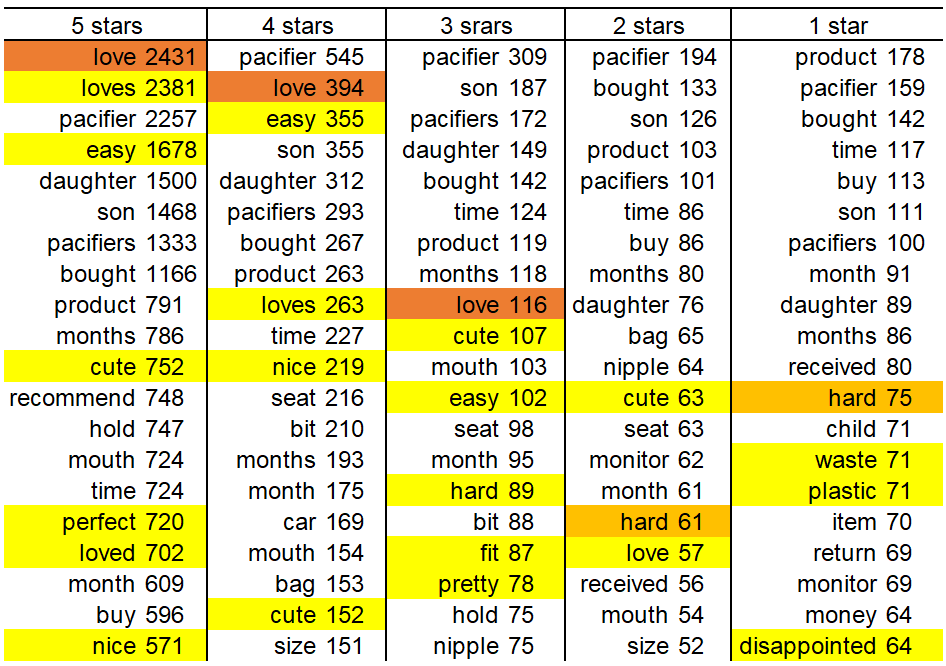
\includegraphics[width=14cm]{./figures/pdc2.png}
	\caption{婴儿奶嘴不同星级所对应的单词频数Top20} \label{pdc1}
\end{figure}

差评是我们真正关注的地方,能从中发现哪些方面消费者有不满,进而对产品或在线销售策略做出调整,提高公司竞争力。从图\ref{pdc1}可知:

1.在评价产品时,消费者更喜欢描述主观感受,而不是产品属性。

2.Specific quality descriptors of text-based reviews such as ‘love’, ‘disappointed’, and others, strongly associated with rating levels.

3.在低星级评分中,"hard","plastic"反应出婴儿奶嘴潜在的重要设计功能是其软硬程度和是材料安全性;吹风机潜在的重要设计功能是烘干效果和是使用寿命。微波炉潜在的重要设计功能是功能多样性和是售后服务。



\subsection{How to Know the Product’s Reputation}
消费者真实评价分数只考虑到了评论内容与星级,没有考虑评论的重要性。在考虑产品声誉时最重要的四个因素是:星级,评论,vine,有用票数。\upcite{WannThe}
每个评论者对该产品的声誉贡献分数$p_{i}$:

\begin{equation}\label{q2}
p_{i}=\sum_{i}^{n_i}[s_{i}+k_{i}(r_{i1}+r_{i2})]
\end{equation}

一个产品的声誉考虑到某一点时间内每个评论者对该产品的声誉打分,得到如下指标。该指标可以描述产品在某一段时间的声誉情况,是下降还是上升,其中$n_k$为j产品在第k个月内的评论个数。j产品的第k个月声誉得分$rp_{jk}$:

\begin{equation}\label{gs1}
rp_{jk}=\frac{\sum_{i}^{n_k}[s_{ji}+k_{ji}(r_{ji1}+r_{ji2})]}{n_i}
\end{equation}

在进行画图表示时,我们将数据做了一些处理:每个评论者对该产品的声誉分$rp_{i}$通过把它转化为$[-1,1]$上的数。$(0,1]$上的值表示每个评论者对该产品的声誉贡献分是正向的;$[-1,0)$上的值表示每个评论者对该产品的声誉贡献分是负向的;0表示每个评论者对该产品没有声誉贡献分;因为婴儿安抚奶嘴的数据最多有18939条,所以我们挑选的数据是安抚奶嘴的数据。

\begin{figure}[H]
	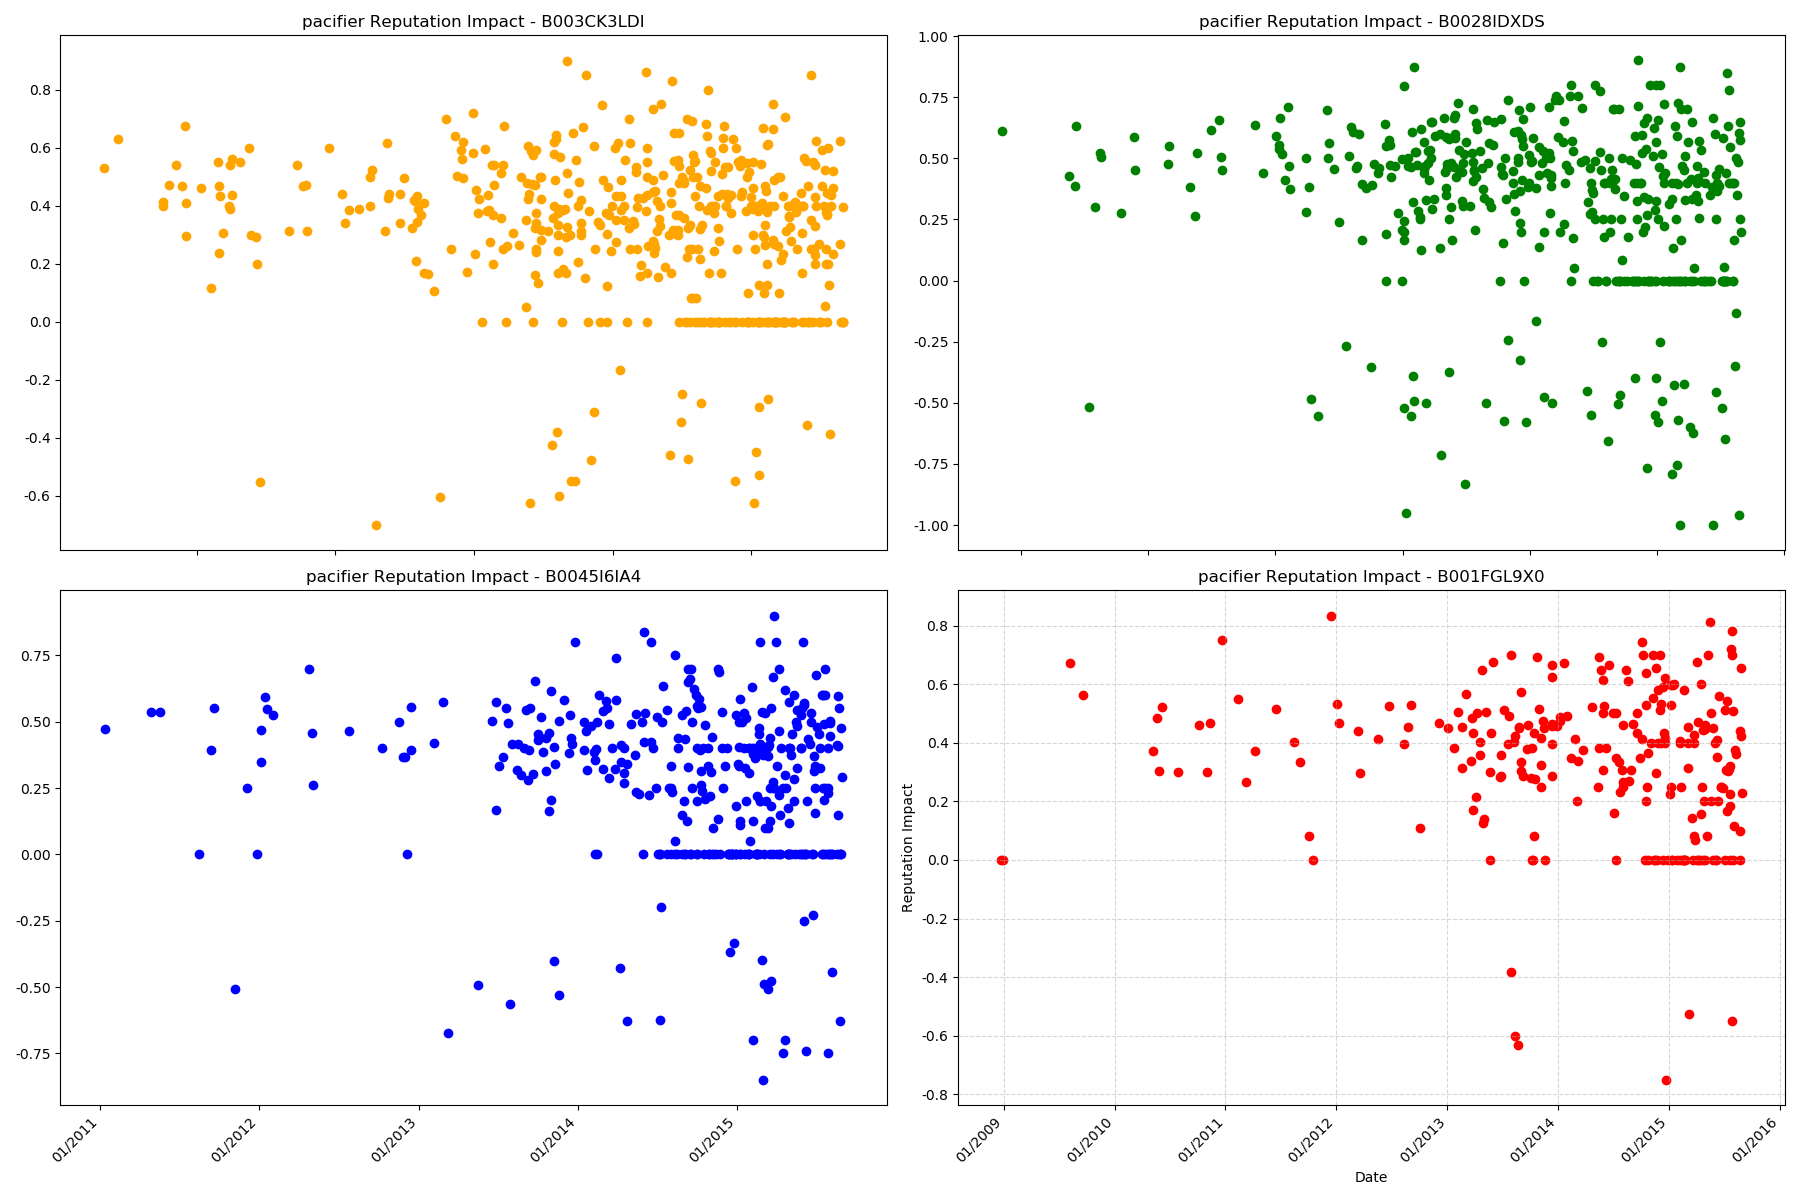
\includegraphics[width=7cm]{./figures/q2p1p.png}
	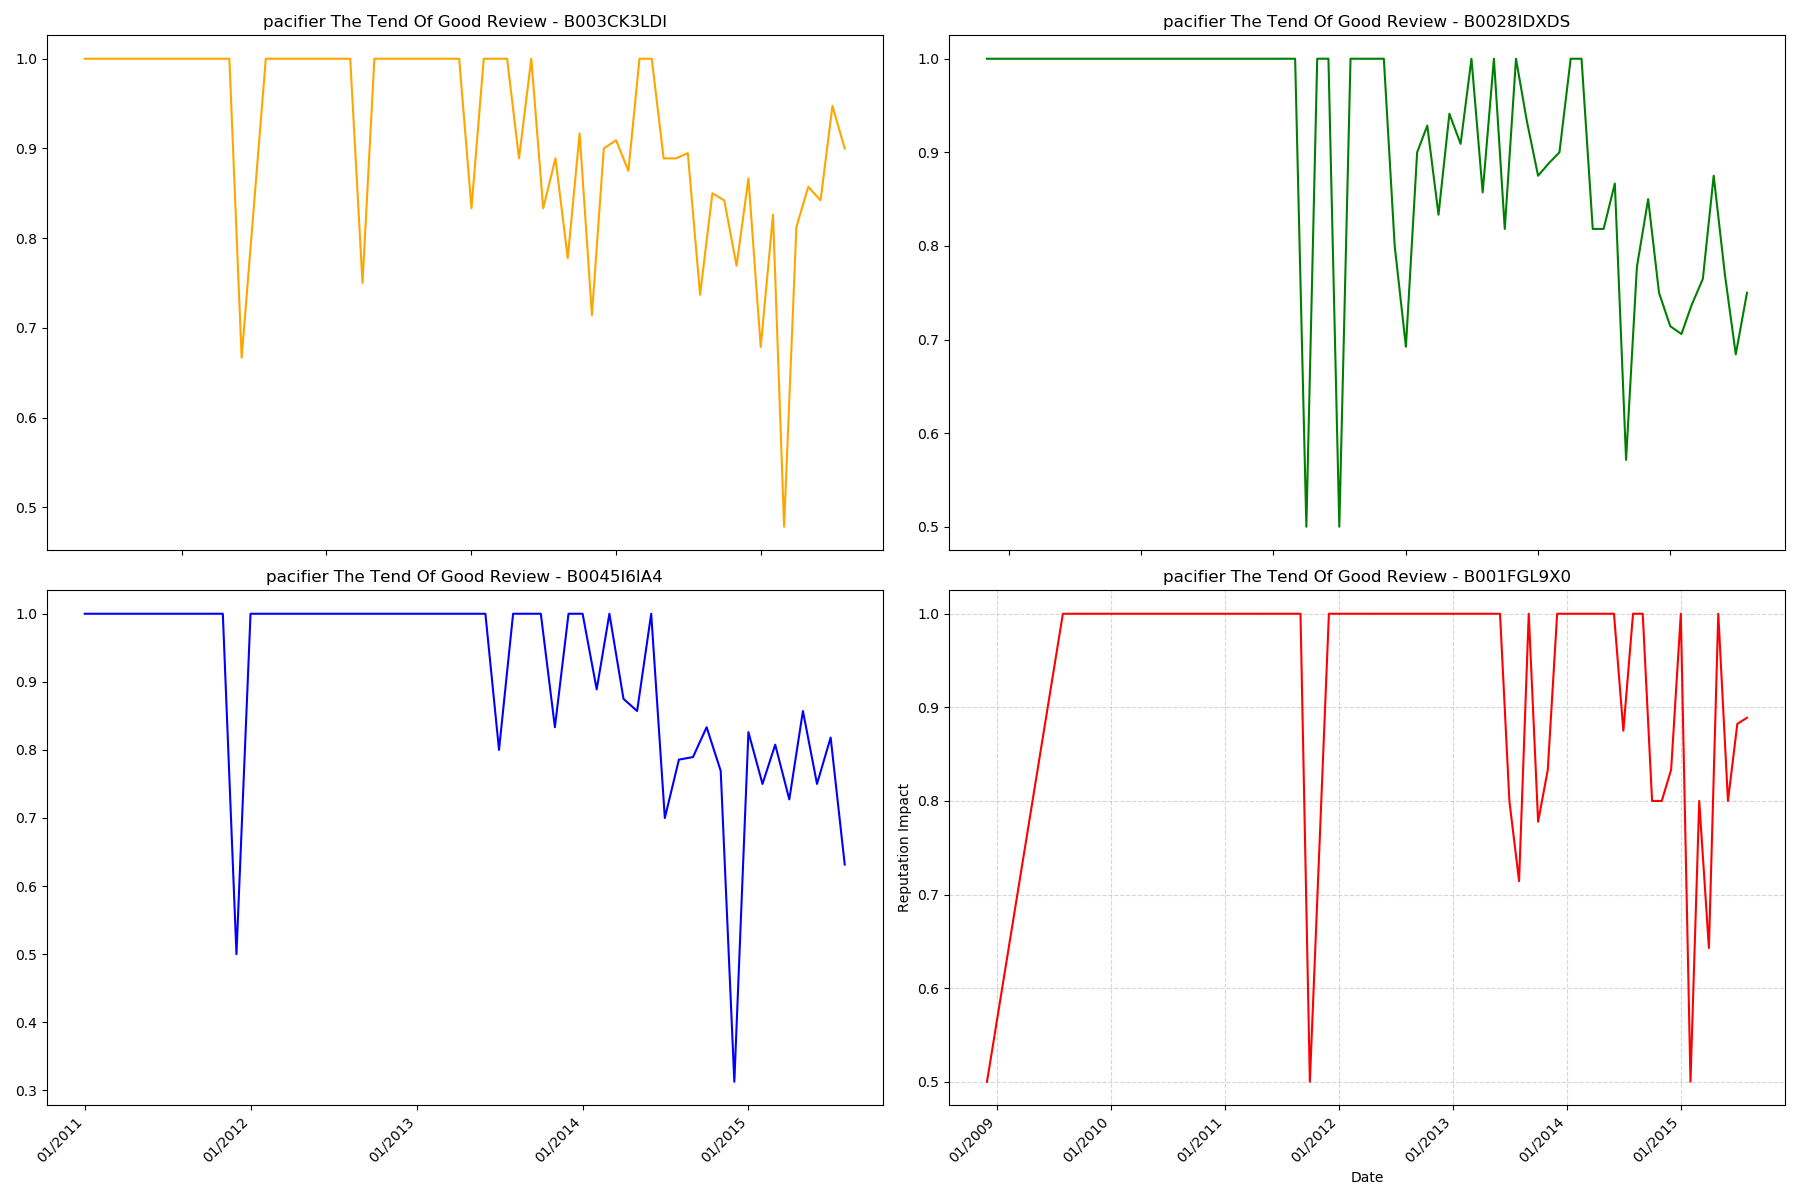
\includegraphics[width=7cm]{./figures/q2p2p.png}
	\caption{左图:婴儿安抚奶嘴数据中评论数量排名前四的产品的每个评论者对该产品的声誉分;右图:婴儿安抚奶嘴数据中评论数量排名前四的产品的在每月的声誉得分} \label{q2p1}
\end{figure}

图\ref{q2p1}左图可知评论数量排名前四的产品的声誉得分绝大多数集中在0上方,这说明大多数人对产品的评价是积极的的(与图\ref{z1_q1p1}右图得出结论一致)。这里我们选取的是评论数量排名前四的产品,所以这些产品销售量同样很高。

图\ref{q2p1}右图研究的是一个月中五星评论数量论占评论总数的比例。声誉得分都是稳定在0.5以上的,偶尔该月评论中全是五星评论,这对销售公司非常有利。2015年前后声誉发生突变,后又趋于稳定状态。因为随着网上购物越来越普遍,评论数据不断增加,购物平台上不可对每一条评论都进行显示,所以网络公司对购物平台评论显示做出相应调整。

综上所述,销量与声誉是紧密相关的,我们在此强烈建议阳光公司一点要注重产品的声誉。

\subsection{how to know  the future trend of the product }
一个产品在在线市场销售后,怎么定义它的成功?如果该产品有很多人购买,购买后的评论大多数是积极的,并且产品在网络上的声誉是良好,那么产品未来的趋势一定是向好的方向发展。

\begin{figure}[H]
	\centering
	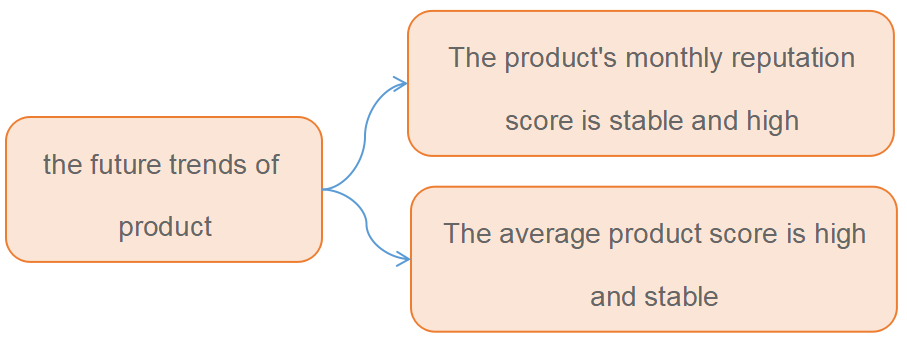
\includegraphics[width=7cm]{./figures/q3p1.png}
	\caption{the combination to indicate a potentially successful or failing product.} \label{q3p11}
\end{figure}

声誉得分和产品得分是影响一个产品未来发展的重要因素。通过公式\ref{zy1}可以知道产品得分$f3_i$是衡量产品质量的综合性指标;通过公式\ref{gs1}可以知道声誉得分会影响产品未来的销售量。这两个指标一个衡量产品的属性好坏,一个体现社会价值,相加在一起就能对产品的未来趋势有全方位的预测。产品未来发展得分$\psi$:
\begin{equation}\label{gs4q1}
\psi_j=\mathbf{avg}\sum (f_{2jk}+rp_{jk})
\end{equation}

\begin{table}[H]	
	\caption{不同产品三种指标的对比}\label{biao4q1}
	\centering
\begin{tabular}{c|cccc}
	\hline &review number & product score  & product reputation  & total  \\
	 product id &$n_j$ & $f_{2j}$ & $rp_{j}$ & $\psi_j$ \\
	\hline B0009XH6TG & 555 & 53.76 & 13.30 & 67.06 \\
	B00VRN7SB8 & 15 & 3.37 & 16.00 & 19.37 \\
	B005GSZB9Q & 78 & 13.53 & 15.42 & 28.95 \\
	B00NXRHIO8 & 13 & 4.57 & 17.62 & 22.18 \\
	B003CK3LDI & 515 & 54.13 & 13.04 & 67.17 \\
	B00UH2XBOS & 14 & 2.65 & 13.31 & 15.96 \\
	\hline
\end{tabular}
\end{table}

从表\ref{biao4q1}可知:评论数量越多的产品具有更高的未来发展得分。因为产品销售的越多评论数量越多,所以评论数量就能间接代表销售数量。如果我们能证明评论数量和未来发展得分是呈正相关关系的,那么就能说明$\psi_j$未来发展得分越高,销售量就会越多,产品越可能成功。

\subsection{Do specific star ratings incite more reviews?}
问题四要求分析客户进行评论时是否会受到产品已有评级的影响,在评论时在情感上产生偏向性。于是我们就来探究用户评价之前,产品以前的一定数量的评级对评论内容情感产生的影响。

我们首先将三类产品的每一款产品的最近购买的10条订单评级的平均数求出来,并筛选掉评价数不足10条的订单,将最近10条订单评级的平均数Rating the average of stars,记为Ras,将它来作为当前订单的时间节点前的一定数量的星级评价所反映的平均情况。然后来探究它和时间节点后的评论情感之间的相关性。为了简化条件,我们使用Polarity的值来表示评论的情感,记为\(K_{i}\),根据上文中提到的,我们将Polarity数据的值根据范围将差评、中评、好评对应。为了使Polarity在数值上和评级对应,我们将公式\ref{m1gs1}产品得分改为:
\begin{equation}\label{q5gs1}
K_i=1.5K_i
\end{equation}

\subsubsection*{典型相关分析}
1936年Hulling提出了典型相关分析,用于揭示两组多元随机变量之间的线性相关关系。为进一步提取间Ras与\(K_{i}\)这两组变量之间的相关性,我们决定采用典型相关分析,它是利用主成分分析思想,分别找出输入变量与输出变量的线性组合,然后讨论线性组合之间的相关关系~\upcite{jj}。

我们首先假设这两组数据服从联合正态分布。

设 \(\mathbf{X}=\left[\begin{array}{l}
\mathbf{X}^{(1)} \\
\mathbf{X}^{(2)}
\end{array}\right]\)服从正态分布 \(N_{p+q}(\boldsymbol{\mu}, \boldsymbol{\Sigma})\),从总体中抽取样本容量为n的样本,得到下列数据矩阵:

\[\mathbf{X}^{(1)}=\left[\begin{array}{cccc}
X_{11}^{(1)} & X_{12}^{(1)} & \cdots & X_{1 p}^{(1)} \\
X_{21}^{(1)} & X_{22}^{(1)} & \cdots & X_{2 p}^{(1)} \\
\vdots & \vdots & \ddots & \vdots \\
X_{n 1}^{(1)} & X_{n 2}^{(1)} & \cdots & X_{n p}^{(1)}
\end{array}\right]\]

若总体典型相关系数\(\lambda_{k}=0\),则相应的典型变量\(U_{k}\)和 \(V_{k}\)之间无相关关系,因此对于分析\(X^{(1)}\)对\(X^{(2)}\)的影响不起作用.这样的典型变量可以不予考虑,于是提出如何根据样本资料来判断总体典型相关系数是否为零,以便确定应该取几个典型变量的问题。巴特莱特(Bartlett)提出了一个根据样本数据检验总体典型相关系数\(\lambda_{1}, \lambda_{2}, \cdots, \lambda_{r}\)是否等于零的方法。检验假设为

\[\begin{aligned}
&H_{0}: \lambda_{k+1}=\lambda_{k+2}=\cdots=\lambda_{r}=0\\
&H_{1}: \lambda_{k+1} \neq 0
\end{aligned}\]

为了研究RAS和\(K_{i}\)两个指标之间的相关性,我们令RAS为输入变量,\(K_{i}\)的值为输出变量,采用SPSS软件进行求解结果如下:
\begin{table}[H]
	\centering
	\caption{Set 1$\&$ Set2 Standardized Canonical Correlation Coefficients}\label{q4b1}
	\begin{tabular}{cccc}
		\hline Set1 Variable &  & Set2 Variable &  \\
		\hline H polarity & $-0.073$ & H star average & $-0.257$ \\
		P polarity & $-0.991$ & P star average & $-0.946$ \\
		M polarity & $-0.137$ & M star average & $-0.273$ \\
		\hline
	\end{tabular}
\end{table}

然后根据表\ref{q4b1}可以得到第一对Standardized Canonical Correlation Coefficients(标准化的典型相关变量对应的线性组合):

\[\begin{aligned}
&U_{1}^{*}=-0.073 Z_{1}^{(1)}-0.991 Z_{2}^{(1)}-0.137 Z_{3}^{(1)}\\
&V_{1}^{*}=-0.257 Z_{1}^{(2)}-0.946 Z_{2}^{(2)}-0.273 Z_{3}^{(2)}
\end{aligned}\]

其中,\(Z_{i}^{(1)}\)和\(Z_{j}^{(2)}\)分别为原始变量\(X_{i}\)和\(Y_{j}\)标准化后的结果。

以上结果说明P polarity(Pacifier的文本情感评分)在第一组典型相关变量中的重要程度为-0.991,数据的绝对值越大,重要程度越大。P star average(Pacifier的Ras)在第一组典型相关变量中的重要程度为-0.946.同理我们也可以得到两个集合中另外两个变量在第一组典型相关变量中的重要程度。

\begin{table}[H]
	\centering
	\caption{Canonical Correlations}\label{q4b2}
	\begin{tabular}{ccccccc}
		\hline  Correlation & Eigenvalue & Wilks  & $\mathrm{F}$ & $\mathrm{Num} $ & Denom  & Sig. \\
		&  &  Statistic &  & D.F. &  D.F. &  \\
		\hline  0.14 & 0.02 & 0.972 & 2.14 & 9.00 & 1625.89 & 0.024 \\
		0.09 & 0.01 & 0.992 & 1.34 & 4.00 & 1338.00 & 0.254 \\
		0.02 & 0.00 & 0.999 & 0.36 & 1.00 & 670.00 & 0.552 \\
		\hline
	\end{tabular}
\end{table}

从表\ref{q4b2}可以看出第一对典型变量的典型相关系数(Canonical Correlations)中Significance analysis的值为0.024,在\(\alpha\)=0.05的情况下,0.024<0.05,说明在\(95 \%\)的可能性下拒绝原假设,即第一对典型变量的相关性是显著的,说明RAS和K指标存在较强的相关性。第二对和第三对典型变量典型相关系数中Significance analysis的值分别为为0.254和0.552,所以在\(\alpha\) =0.10的情况下,第二三对典型变量间相关性不显著。说明RAS和\(K_{i}\)这两个指标之间只有一对典型变量。

通过典型相关变量的分析,可以得出的结论就是客户评论的内容会受到之前订单评论的星级的影响。

\subsection{ Is the comment content  related to the rating level?}

在探究评论内容和评级的相关性之前,我们先对所有样本数据中的几个定量数据进行描述性统计,以便对数据的特征有大概的了解。
\begin{table}[H]	
	\caption{Descriptive statistics for reviews and ratings and votes}\label{biao5q1}
	\centering
	\begin{tabular}{c|ccc|ccc}
		\hline &&\text { Star Rating } & && \text { Polarity } \\
		& \text {H  } & \text { M } & \text {P  } & \text {H  } & \text {M  } & \text {P  } \\
		\hline \text { Mean } & 4.116 & 3.445 & 4.305 & 0.264 & 0.215 & 0.282 \\
		\text { Standard error} & 0.012 & 0.041 & 0.009 & 0.003 & 0.0068 & 0.002 \\
		\text { Minimum } & 1.000 & 1.000 & 1.000 & -1.000 & -1.000 & -1.000 \\
		\text { Maximum } & 5.000 & 5.000 & 5.000 & 1.000 & 1.000 & 1.000 \\
		\hline
	\end{tabular}
\end{table}

从表\ref{biao5q1}中可以看出,在产品评级方面,三个产品中Pacifier的平均评级最高,Microwave的平均评级最低。在评论类型方面,从它们的平均值来看,买Pacifier的消费者评论内容极值的平均值更高,它们更倾向于给这类产品好评。买Microwave的消费者极值的平均值最低。这一定程度体现出了评级和评价内容类型之间的正相关关系。同时Pacifier产品评级和评论类型的标准差在三类产品中最小,说明这两类数据中的大部分数值和其平均值之间差异较小,数据比较稳定。而三类产品的产品评级和产品评论的最大最小值都没有显著差异。

然后我们来开始探究评论内容和评级的相关性。

从图\ref{q5p1}可以看出,在pacifier产品数据的百分比柱状图中,随着评级的升高,好评数量在总评论数中所占的比例逐渐升高,差评数量在总的评论数量所占的比重逐渐降低。可以看出评级和评论内容有一定的相关性,高评级订单的评论大概率客户给的也是好评,低评级订单的评论中评论内容为差评的可能性也越大。并且中评在五种评级中所占比例都是最低的,说明消费者更倾向于给出极端的评论,极端好评又占大多数,其他两类产品也符和这个特征。

\begin{figure}[H]
	\centering
	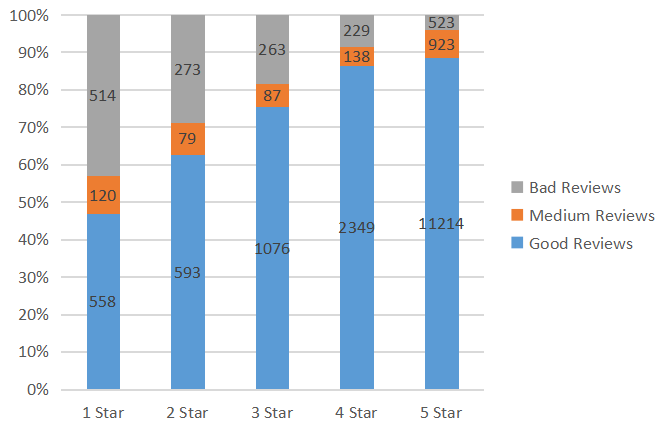
\includegraphics[width=8cm]{./figures/q5p1.png}
	\caption{Pacifier product rating and review type percentage histogram} \label{q5p1}
\end{figure}



本节模型主要是研究评论的极值和评级这两组变量之间的相关关系,我们在excel中统计了我们用TextBlog得到的Polarity数据。我们统计出了三类产品在不同评级的三种评论类型的数量。计算数据的Person相关系数,希望得到评论类型和评级之间的相关关系。Person相关系数计算的公式如下:
\begin{equation}\rho_{X Y}=\frac{\operatorname{Cov}(X, Y)}{\sigma_{X} \sigma_{Y}}=\frac{\sum_{i=1}^{n} \frac{\left(X_{i}-E(X)\right)}{\sigma_{X}} \frac{\left(Y_{i}-E(Y)\right)}{\sigma_{Y}}}{n}
\end{equation}
利用样本数据来计算$\rho_{X Y}$的值,其取值范围在-1到1之间。$\rho_{XY}$>0表示两变量间存在正的相关关系,反之则为负相关关系;$\rho_{XY}$=0表示变量间不存在相关关系;|$\rho_{XY}$|>0.8表示变量间具有较强的相关关系,|$\rho_{XY}$|<0.3表示变量间的相关关系极弱,可认为不相关\upcite{w2}。

\begin{figure}[H]
	\centering
	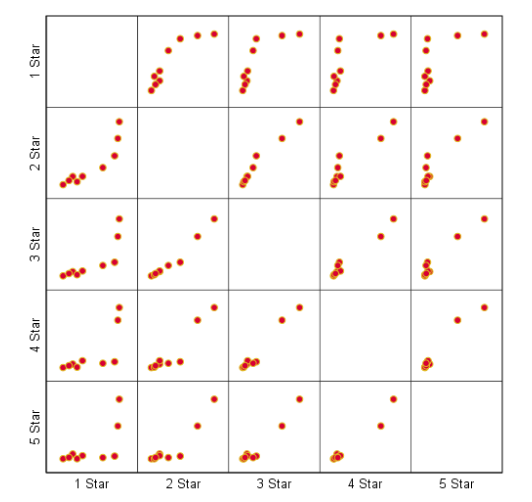
\includegraphics[width=7cm]{./figures/q5p2.png}
	\caption{Pacifier product rating and review type percentage histogram} \label{q5p2}
\end{figure}

每一星级的数据由好评中评差评三种类型的数据构成,通过图\ref{q5p2}可以看出不同星级里面的数据有着较强的正相关关系。然后我们通过计算皮尔逊相关系数来探究文本评论内容和Star Rating的相关关系。

\begin{table}[H]
	\caption{Correlation results}\label{q5b1}
	\centering
	\begin{threeparttable}
	\begin{tabular}{c|ccccc}
		\hline & 1 star & 2 star & 3 star & 4 star & 5star \\
		\hline 1star & 1.00000 & $0.89767^{* *}$ & $0.81339^{* *}$ & $0.73236^{*}$ & $0.66760^{*}$ \\
		2star & $0.89767^{* *}$ & 1.00000 & $0.98154^{* *}$ & $0.94018^{* *}$ & $0.92027^{* *}$ \\
		3star & $0.81339^{* *}$ & $0.98154^{* *}$ & 1.00000 & $0.98349^{* *}$ & $0.97387^{* *}$ \\
		4star & $0.73236^{*}$ & $0.94018^{* *}$ & $0.98349^{* *}$ & 1.00000 & $0.97954^{* *}$ \\
		5star & $0.66760^{*}$ & $0.92027^{* *}$ & $0.97387^{* *}$ & $0.97954^{* *}$ & 1.00000 \\
		\hline								
	\end{tabular}
\begin{tablenotes}
	\footnotesize
	\item[1] \(* *.\)Correlation is significant at the 0.01 level (2-tailed). 
	\item[2] \(*.\)Correlation is significant at the 0.05 level (2-tailed).
\end{tablenotes}
\end{threeparttable}
\end{table}

从表\ref{q5b1}可以看出:各变量间的相关关系都比较大,绝对值均在0.65以上,可以认为变量之间都有较强的正相关关系。其中只有Star Rating为1的数据和Star Rating为4和5的数据相关性相对弱一点,在\(95 \%\)的水平上显著。而其他各个Star Rating的变量之间的相关关系都更强,在\(99 \%\)的水平上显著。此外还可以看出,Star Rating为1星的数据和其他数据的相关性,随着Star Rating数据星级的升高,Star Rating为1星的数据和其他数据的相关性逐渐降低。Star Rating为5星的数据也有类似的关系,它和其他数据的相关性随着Star Rating数据星级从1星开始升高,Star Rating为5星的数据和其他数据的相关性逐渐增加。

这首先说明了消费者对产品打的不同评级,它们的评价内容的3种类型的数据之间的相关性都比较强。而评级为1星和评级为5星的订单它们的评论内容类型之间的相关性要相对低一些点。

\section*{模型改进}
停用词的选择上,将"good","great","n't"不作为停用词,得到单词频率与频数。我们将更新图\ref{wordCloud}和图\ref{pdc1}。在解题思路的展现方式上,可以选用不同星级所对应的不同词性的单词频数,分别了解动词,形容词,名词的出现频数,这将更有利于我们对产品情况的分析。

在讨论产品未来趋势时,我们得到了产品未来发展的分。在本文中只对部分数据进行了展示,还应建立评论数量与产品未来发展得分线性模型,对其相关性做出检验,找到评论数量与评论数量与产品未来发展得分两者之间的对应关系。

\section*{敏感性分析}
 本文中有关星级,评论有效分数,评价得分在消费者真实评价分数与商品得分中的权重是一个固定值。但我们知道由于不同的消费者影响可能会有所不同,因此应对面对的两个目标活动 (销售策略和产品设计功能)的权重和实际情况
相联系。因此,我们针对$0.1,0.2,\cdots,i$计算 10 组结果,以测试模型的敏感性和可行性。消费者真实评价分数中,$\phi=0.4$ 和$\phi=0.6$之间有很大的跳跃;商品得分中介于$\phi=0.2$ 和$\phi=0.4$之间。参数的值接近这些阈值时,计算结果几乎不受影响。但是,当该值远离阈值时,灵敏度非常高。因此,$\phi$和$\eta$应该根据实际情况,尤其是当该值接近阈值时。

\section*{模型优缺点}
\subsection*{优点}
1) 较为全面、客观的指标

在寻找和选择关于产品的指标时,我们尽可能全面、细致地考虑它的等式。与数据集中大部分的指标都关联了起来,这意味着我们的模型是有效的、有意义的基础。

2)模型比较正确的结果

在指标和数据数量有限的情况下,模型的结果仍较为符合客观事实。特别地,结果突出了产品得分、产品信誉等多项度量对产品成功的影响,这是新颖和有效的。
3)广泛的度量模式

在我们的模型中,根据星级评分、帮助评分、评论内容三个方面选取度量,设计了反映产品得分、产品声誉、产品潜力等多方面的度量。

4)直观的结果

在不同的模型中,我们大量的使用了图表的形式去展现我们的分析和结果,并采取了新颖的方式去展现,如词语图,这可以更为直观的了解产品相关参数变化的趋势。

5)较好的可扩展性

对数据集的数据挖掘和分析及时间序列图的绘制,均有Python 代码完成,具有极高的可扩展性。如停用词的选择上,我们可以根据自己实际情况对其进行了修正,包括停用词和关键字的选择等待,使得结果会更加精准。

\subsection{缺点}
1) 指标选择过程中的主观性和局限性。

虽然参考了相关文献以及客观事实的影响因素,但仍然选择了具有主观概
念的指标。但没有足够的文献与全面的数据,这是不可避免的。

2)时间的不连续性带来的误差。

由于数据的时间并不连续,所以对于时间的度量只是一个大概的范围

3)数据的局限性

在对数据分析中,我们只评估了数据集中的状况,日期相当有限。以这种方式,我们的分析结果不够全面和精确,不足以代表所有商品在网上的销售策略。由于使用的是历史数据集,如果未来网上销售出现新的变化或热潮,此模型可能并不适用。




\addcontentsline{toc}{section}{Reference}
%\nocite{Bibtexkey}
\bibliographystyle{plain}
\bibliography{myreference}


\end{document}